\section{Delaunay Triangulation}

\subsection{What Is a Triangulation?}

Given a set of distinct points $P = \{p_1, p_2, \dots, p_N\}$ in the plane $\mathbb{R}^2$,
a \emph{triangulation} is a subdivision of the convex hull of $P$ into triangles such that:
\begin{itemize}
    \item every triangle vertex is a point from $P$,
    \item the interiors of any two triangles do not intersect,
    \item the union of all triangles equals the convex hull of $P$.
\end{itemize}

In other words, a triangulation connects the given points with non-crossing edges
to form a tiling of triangles covering the entire convex hull, leaving no gaps
or overlaps.  A single point set typically admits many different triangulations.
Figure~\ref{fig:triang-comparison} shows two valid triangulations of the same
point set---they use identical vertices but different edge connections.

\begin{figure}[htbp]
    \centering
    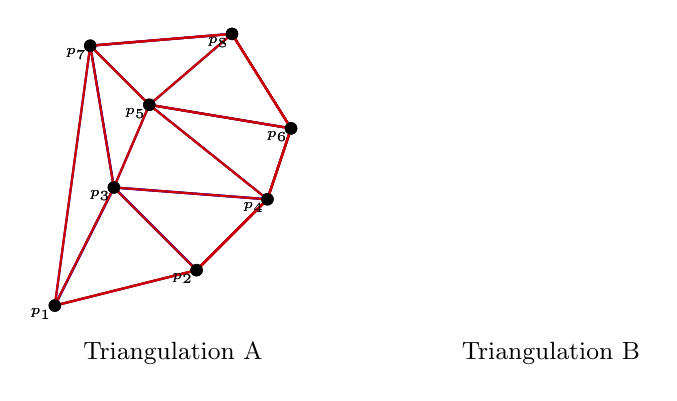
\begin{tikzpicture}[scale=1.5]
        % Point positions
        \coordinate (A) at (0, 0);
        \coordinate (B) at (1.2, 0.3);
        \coordinate (C) at (0.5, 1.0);
        \coordinate (D) at (1.8, 0.9);
        \coordinate (E) at (0.8, 1.7);
        \coordinate (F) at (2.0, 1.5);
        \coordinate (G) at (0.3, 2.2);
        \coordinate (H) at (1.5, 2.3);

        % --- Left: Triangulation 1 ---
        \begin{scope}[xshift=0cm]
            \draw[gray!60, thin] (A) -- (B) -- (D) -- (F) -- (H) -- (G) -- cycle;
            \draw[blue!80!black, thick] (A) -- (B) -- (D) -- (F) -- (H) -- (G) -- cycle;
            \draw[blue!80!black, thick] (A) -- (C) -- (B);
            \draw[blue!80!black, thick] (A) -- (C) -- (G);
            \draw[blue!80!black, thick] (B) -- (C) -- (E);
            \draw[blue!80!black, thick] (B) -- (D) -- (C);
            \draw[blue!80!black, thick] (C) -- (D) -- (E);
            \draw[blue!80!black, thick] (C) -- (G) -- (E);
            \draw[blue!80!black, thick] (D) -- (F) -- (E);
            \draw[blue!80!black, thick] (E) -- (F) -- (H);
            \draw[blue!80!black, thick] (E) -- (H) -- (G);

            \foreach \pt/\lbl in {A/$p_1$,B/$p_2$,C/$p_3$,D/$p_4$,E/$p_5$,F/$p_6$,G/$p_7$,H/$p_8$}
            {
                \fill[black] (\pt) circle (1.5pt);
                \node[anchor=north east, font=\tiny, inner sep=1pt] at (\pt) {\lbl};
            }
            \node at (1.0, -0.4) {\small Triangulation A};
        \end{scope}

        % --- Right: Triangulation 2 ---
        \begin{scope}[xshift=3.2cm]
            \draw[gray!60, thin] (A) -- (B) -- (D) -- (F) -- (H) -- (G) -- cycle;
            \draw[red!80!black, thick] (A) -- (B) -- (D) -- (F) -- (H) -- (G) -- cycle;
            \draw[red!80!black, thick] (A) -- (C) -- (G);
            \draw[red!80!black, thick] (A) -- (B) -- (C);
            \draw[red!80!black, thick] (B) -- (D) -- (C);
            \draw[red!80!black, thick] (B) -- (D) -- (E);
            \draw[red!80!black, thick] (C) -- (E) -- (G);
            \draw[red!80!black, thick] (D) -- (F) -- (E);
            \draw[red!80!black, thick] (D) -- (F) -- (H);
            \draw[red!80!black, thick] (E) -- (F) -- (H);
            \draw[red!80!black, thick] (E) -- (H) -- (G);

            \foreach \pt/\lbl in {A/$p_1$,B/$p_2$,C/$p_3$,D/$p_4$,E/$p_5$,F/$p_6$,G/$p_7$,H/$p_8$}
            {
                \fill[black] (\pt) circle (1.5pt);
                \node[anchor=north east, font=\tiny, inner sep=1pt] at (\pt) {\lbl};
            }
            \node at (1.0, -0.4) {\small Triangulation B};
        \end{scope}
    \end{tikzpicture}
    \caption{Two different valid triangulations of the same eight-point set.
    The convex hull edges (darker) are the same in both, but the internal
    edges differ, yielding different triangle shapes and qualities.}
    \label{fig:triang-comparison}
\end{figure}

For $N$ points in \emph{general position} (no three collinear), the number of
triangles and edges in any triangulation is fixed.  If $h$ of the $N$ points lie
on the convex hull boundary, then every triangulation has exactly
\[
    T = 2N - 2 - h \quad \text{triangles}
    \qquad\text{and}\qquad
    E = 3N - 3 - h \quad \text{edges}.
\]
When the points are well distributed (roughly $h \approx \sqrt{N}$), this is
approximately $2N$ triangles and $3N$ edges.  The counting follows from Euler's
formula for planar graphs: $V - E + F = 1 + C$, where for a triangulation
$V = N$, each internal face is a triangle, and $C = 1$ for a connected graph.

\subsection{Why Triangulation in Face Morphing?}

In feature-based face morphing, we place landmark points on key facial features
(eyes, nose, mouth contour, jawline, etc.) in both source and target images.
The next step is \emph{warping}: moving pixels from the source image to their
corresponding positions in the target.  Triangulation provides the geometric
framework for this warp.

Each triangle in the source triangulation maps to a corresponding triangle in
the target triangulation via an \emph{affine transformation}.  Affine transforms
preserve lines and ratios of distances, so lines inside a triangle remain lines
after warping---a critical property for avoiding visible seams.

Triangles are the ideal choice for several reasons:
\begin{enumerate}
    \item \textbf{Uniqueness of the transform.} Three non-collinear points
    uniquely determine an affine transformation.  Given source triangle
    $(a, b, c)$ and target triangle $(a', b', c')$, there is exactly one
    affine map $T$ with $T(a)=a'$, $T(b)=b'$, $T(c)=c'$.
    \item \textbf{Planarity.} A triangle is always planar---its three vertices
    always lie in a single plane.  Under an affine transformation, the image of
    a triangle is always another triangle, never a self-intersecting shape.
    \item \textbf{Complete partitioning.} A triangulation covers the convex hull
    entirely, with no gaps between triangles and no overlaps (except shared
    edges).  Every pixel inside the hull belongs to exactly one triangle.
    \item \textbf{Why not quadrilaterals or higher polygons?} A quadrilateral
    is not necessarily planar under an affine transform---its four vertices may
    map to a non-planar configuration that cannot be represented by a single
    affine map in 2D.  One could subdivide a quadrilateral into two triangles,
    but then we are back to triangulation.  Higher-order polygons have the same
    problem, worsened.
\end{enumerate}

The quality of the triangulation directly affects the visual quality of the
morph.  Long, thin (``skinny'') triangles produce highly non-uniform stretches
that look visibly distorted.  This motivates choosing a triangulation that
avoids skinny triangles---which brings us to the Delaunay triangulation.

\subsection{The Delaunay Triangulation}

\begin{definition}[Circumcircle]
    The \emph{circumcircle} of a triangle is the unique circle passing through
    all three of its vertices.  Every non-degenerate triangle has exactly one
    circumcircle.  The center of the circumcircle (the \emph{circumcenter}) is
    the intersection of the three perpendicular bisectors of the triangle's edges.
\end{definition}

\begin{theorem}[Empty Circumcircle Property]
    Given a set of points $P \subset \mathbb{R}^2$, the \emph{Delaunay
    triangulation} $DT(P)$ is the unique triangulation of $P$ satisfying the
    following property: for every triangle $\triangle abc$ in $DT(P)$, the open
    interior of its circumcircle contains no point of $P$.
\end{theorem}

Equivalently, no point of $P$ lies strictly inside the circumcircle of any
triangle in the Delaunay triangulation.  Points may lie \emph{on} the
circumcircle (this happens precisely when four or more points are co-circular),
but never strictly inside.

\begin{figure}[htbp]
    \centering
    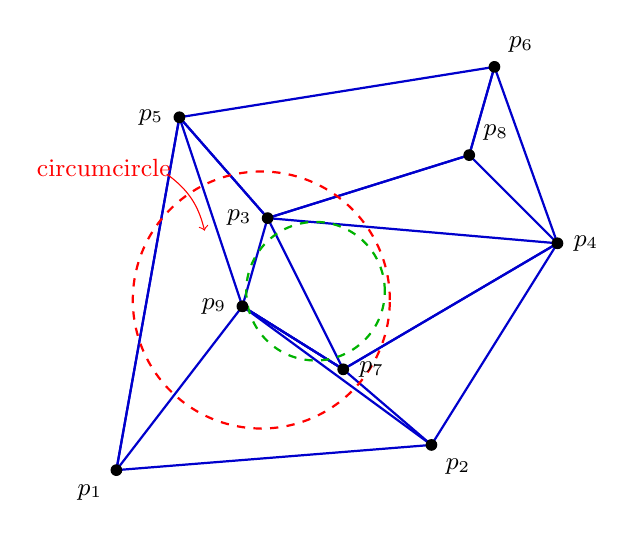
\begin{tikzpicture}[scale=1.6]
        % Define points
        \coordinate (A) at (0, 0);
        \coordinate (B) at (2.5, 0.2);
        \coordinate (C) at (1.2, 2.0);
        \coordinate (D) at (3.5, 1.8);
        \coordinate (E) at (0.5, 2.8);
        \coordinate (F) at (3.0, 3.2);
        \coordinate (G) at (1.8, 0.8);
        \coordinate (H) at (2.8, 2.5);
        \coordinate (I) at (1.0, 1.3);

        % Delaunay triangulation edges
        \draw[blue!80!black, thick] (A) -- (B) -- (D) -- (F) -- (E) -- cycle;
        \draw[blue!80!black, thick] (A) -- (I) -- (B);
        \draw[blue!80!black, thick] (A) -- (E) -- (I);
        \draw[blue!80!black, thick] (I) -- (G) -- (B);
        \draw[blue!80!black, thick] (I) -- (G) -- (D);
        \draw[blue!80!black, thick] (I) -- (G) -- (C);
        \draw[blue!80!black, thick] (I) -- (C) -- (E);
        \draw[blue!80!black, thick] (G) -- (D) -- (C);
        \draw[blue!80!black, thick] (C) -- (H) -- (D);
        \draw[blue!80!black, thick] (C) -- (H) -- (F);
        \draw[blue!80!black, thick] (C) -- (E);
        \draw[blue!80!black, thick] (H) -- (F);

        % Highlight one triangle with circumcircle
        \coordinate (O1) at (1.15, 1.35); % approximate circumcenter of A, I, E
        \pgfmathsetmacro{\rOne}{1.02}

        \draw[red, dashed, thick] (O1) circle (\rOne);

        % Circumcircle of I, G, C
        \coordinate (O2) at (1.58, 1.42);
        \pgfmathsetmacro{\rTwo}{0.55}
        \draw[green!70!black, dashed, thick] (O2) circle (\rTwo);

        % Points
        \foreach \pt/\lbl/\pos in {
            A/$p_1$/below left,
            B/$p_2$/below right,
            C/$p_3$/left,
            D/$p_4$/right,
            E/$p_5$/left,
            F/$p_6$/above right,
            G/$p_7$/right,
            H/$p_8$/above right,
            I/$p_9$/left
        } {
            \node[circle, fill=black, inner sep=1.5pt, label={\pos:\small\lbl}] at (\pt) {};
        }

        % Label highlighting circumcircle
        \node[red, font=\small] at (-0.1, 2.4) {circumcircle};
        \draw[red, ->] (0.4, 2.35) to [bend left=20] (0.7, 1.9);
    \end{tikzpicture}
    \caption{Delaunay triangulation of a nine-point set.  The red dashed circle
    is the circumcircle of one triangle; notice that no other points lie
    strictly inside it.  This is the defining \emph{empty circumcircle property}
    of the Delaunay triangulation.}
    \label{fig:delaunay-circumcircle}
\end{figure}

\paragraph{Connection to the Voronoi Diagram.}
The Delaunay triangulation is closely related to the Voronoi diagram.
Given $P = \{p_1, \dots, p_N\}$, the Voronoi cell of $p_i$ is the region of
the plane consisting of all points closer to $p_i$ than to any other point:
\[
    V(p_i) = \{\, x \in \mathbb{R}^2 \mid \|x - p_i\| \leq \|x - p_j\|
    \text{ for all } j \neq i \,\}.
\]
The \emph{Voronoi diagram} is the subdivision of the plane into these cells.
The Delaunay triangulation is the \emph{dual graph} of the Voronoi diagram:
two points $p_i$ and $p_j$ are connected by a Delaunay edge if and only if
their Voronoi cells $V(p_i)$ and $V(p_j)$ share a boundary segment.  This
duality provides both geometric intuition and practical algorithms: computing
the Voronoi diagram immediately yields the Delaunay triangulation and vice versa.

\subsection{Key Properties of Delaunay Triangulation}

The Delaunay triangulation is preferred over arbitrary triangulations because
of several optimality properties.

\subsubsection*{Max--Min Angle Property}

\begin{theorem}[Max--Min Angle]
    Among all possible triangulations of a given point set, the Delaunay
    triangulation maximizes the minimum interior angle across all triangles.
    That is, if $\alpha_{\min}(T)$ denotes the smallest interior angle in
    triangulation $T$, then
    \[
        \alpha_{\min}(DT(P)) \geq \alpha_{\min}(T)
        \quad \text{for all triangulations } T \text{ of } P.
    \]
\end{theorem}

This property is crucial for face morphing.  Triangles with very small angles
are ``skinny''---they have a large aspect ratio.  When a skinny triangle is
affinely mapped to a better-shaped target triangle, the mapping stretches
pixels enormously in one direction and compresses them in another, producing
visible artifacts.  The max--min angle guarantee ensures that Delaunay
triangles are as ``equilateral as possible,'' minimizing distortion.

\subsubsection*{Uniqueness}

\begin{proposition}
    If no four points of $P$ lie on a common circle (the \emph{general
    position} assumption), then the Delaunay triangulation of $P$ is unique.
\end{proposition}

When four or more points are co-circular, there can be multiple valid Delaunay
triangulations.  For example, four points forming a rectangle all lie on a
common circle; the diagonal can be chosen either way and both triangulations
satisfy the empty circumcircle property.  In practice with real-valued landmark
coordinates, co-circularity is extremely unlikely.

\subsubsection*{Local (Incremental) Property}

An important practical property is that the Delaunay triangulation can be
constructed incrementally.  Given $DT(\{p_1, \dots, p_k\})$, inserting a new
point $p_{k+1}$ requires modifying only the triangles whose circumcircles
contain $p_{k+1}$.  All other triangles remain unchanged.  This is the key
insight behind many efficient Delaunay construction algorithms.

\subsection{The Bowyer--Watson Algorithm}

The Bowyer--Watson algorithm is an incremental algorithm for constructing the
Delaunay triangulation.  It was published independently by Bowyer (1981) and
Watson (1981), and is widely used in practice due to its simplicity and
robustness.

\subsubsection*{Algorithm Steps}

\begin{enumerate}
    \item \textbf{Create a super-triangle.} Start with an artificial triangle
    large enough to contain all input points.  This avoids boundary-condition
    complications during incremental insertion.
    \item \textbf{Insert points one at a time.} For each point $p$:
    \begin{enumerate}
        \item \textbf{Find bad triangles.} Identify all existing triangles
        whose circumcircles contain $p$.  These triangles violate the empty
        circumcircle property and must be removed.
        \item \textbf{Find the cavity boundary.} The removed triangles create
        a polygonal hole (the \emph{cavity}).  Find the unique polygon edges
        on the boundary of this hole---edges that belong to exactly one removed
        triangle (the other side is part of the hole interior).
        \item \textbf{Re-triangulate.} Connect $p$ to each vertex of the
        cavity boundary, forming new triangles.  Each new triangle has $p$ as
        one vertex and a cavity boundary edge as the opposite side.
    \end{enumerate}
    \item \textbf{Remove super-triangle artifacts.} After all points have been
    inserted, discard any triangle that shares a vertex with the original
    super-triangle.
\end{enumerate}

\begin{figure}[htbp]
    \centering
    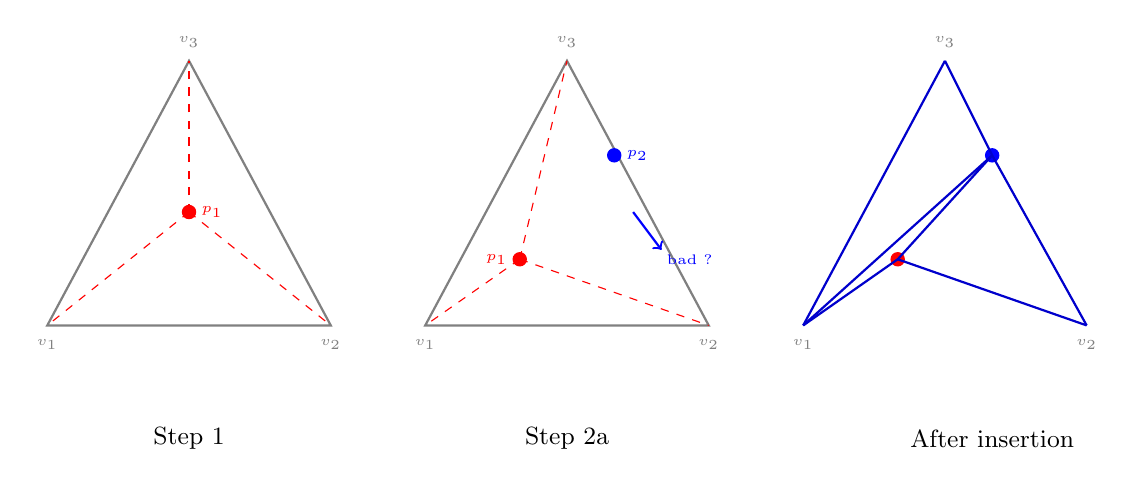
\begin{tikzpicture}[scale=1.2]
        % Step 1: Super-triangle with one point
        \begin{scope}[xshift=0cm]
            \node[font=\small] at (1.5, -1.2) {Step 1};
            \draw[gray, thick] (0, 0) -- (3, 0) -- (1.5, 2.8) -- cycle;
            \node[gray, font=\tiny] at (0, -0.2) {$v_1$};
            \node[gray, font=\tiny] at (3, -0.2) {$v_2$};
            \node[gray, font=\tiny] at (1.5, 3.0) {$v_3$};
            \filldraw[red] (1.5, 1.2) circle (2pt) node[right=1pt] {\tiny $p_1$};
            \draw[red, dashed] (1.5, 1.2) -- (0, 0);
            \draw[red, dashed] (1.5, 1.2) -- (3, 0);
            \draw[red, dashed] (1.5, 1.2) -- (1.5, 2.8);
        \end{scope}

        % Step 2: Add second point, find bad triangle
        \begin{scope}[xshift=4cm]
            \node[font=\small] at (1.5, -1.2) {Step 2a};
            \draw[gray, thick] (0, 0) -- (3, 0) -- (1.5, 2.8) -- cycle;
            \node[gray, font=\tiny] at (0, -0.2) {$v_1$};
            \node[gray, font=\tiny] at (3, -0.2) {$v_2$};
            \node[gray, font=\tiny] at (1.5, 3.0) {$v_3$};
            \filldraw[red] (1.0, 0.7) circle (2pt) node[left=1pt] {\tiny $p_1$};
            \filldraw[blue] (2.0, 1.8) circle (2pt) node[right=1pt] {\tiny $p_2$};

            \draw[red, dashed] (1.0, 0.7) -- (0, 0);
            \draw[red, dashed] (1.0, 0.7) -- (3, 0);
            \draw[red, dashed] (1.0, 0.7) -- (1.5, 2.8);

            \draw[blue, ->, thick] (2.2, 1.2) -- (2.5, 0.8);
            \node[blue, font=\tiny] at (2.8, 0.7) {bad ?};
        \end{scope}

        % Step 3: After insertion
        \begin{scope}[xshift=8cm]
            \node[font=\small] at (2.0, -1.2) {After insertion};
            \filldraw[red] (1.0, 0.7) circle (2pt);
            \filldraw[blue] (2.0, 1.8) circle (2pt);
            \draw[blue!80!black, thick] (0, 0) -- (1.0, 0.7);
            \draw[blue!80!black, thick] (3, 0) -- (1.0, 0.7);
            \draw[blue!80!black, thick] (1.0, 0.7) -- (2.0, 1.8);
            \draw[blue!80!black, thick] (2.0, 1.8) -- (0, 0);
            \draw[blue!80!black, thick] (2.0, 1.8) -- (3, 0);
            \draw[blue!80!black, thick] (1.5, 2.8) -- (0, 0);
            \draw[blue!80!black, thick] (1.5, 2.8) -- (2.0, 1.8);
            \node[gray, font=\tiny] at (0, -0.2) {$v_1$};
            \node[gray, font=\tiny] at (3, -0.2) {$v_2$};
            \node[gray, font=\tiny] at (1.5, 3.0) {$v_3$};
        \end{scope}
    \end{tikzpicture}
    \caption{Illustration of the Bowyer--Watson algorithm inserting two points
    into a super-triangle.  Each new point identifies the triangles whose
    circumcircles contain it, removes them, and re-triangulates the cavity.}
    \label{fig:bowyer-watson}
\end{figure}

\subsubsection*{Pseudocode}

\begin{algorithm}[H]
\caption{Bowyer--Watson Delaunay Triangulation}
\label{alg:bowyer-watson}
\begin{algorithmic}[1]
\Require A set of points $P = \{p_1, p_2, \dots, p_N\}$
\Ensure Delaunay triangulation $DT(P)$
\State Create a super-triangle $T_{\text{super}}$ containing all points in $P$
\State $\mathcal{T} \gets \{T_{\text{super}}\}$ \Comment{current triangulation}
\For{each point $p \in P$}
    \State $\mathcal{B} \gets \emptyset$ \Comment{bad triangles}
    \For{each triangle $t \in \mathcal{T}$}
        \If{$p$ is inside the circumcircle of $t$}
            \State $\mathcal{B} \gets \mathcal{B} \cup \{t\}$
        \EndIf
    \EndFor
    \State $\mathcal{E}_{\text{boundary}} \gets \emptyset$ \Comment{cavity boundary edges}
    \For{each triangle $t \in \mathcal{B}$}
        \For{each edge $e$ of $t$}
            \If{$e$ is not shared with another triangle in $\mathcal{B}$}
                \State $\mathcal{E}_{\text{boundary}} \gets \mathcal{E}_{\text{boundary}} \cup \{e\}$
            \EndIf
        \EndFor
    \EndFor
    \State $\mathcal{T} \gets \mathcal{T} \setminus \mathcal{B}$
    \For{each edge $(v_i, v_j) \in \mathcal{E}_{\text{boundary}}$}
        \State $\mathcal{T} \gets \mathcal{T} \cup \{\triangle(v_i, v_j, p)\}$
    \EndFor
\EndFor
\State Remove all triangles from $\mathcal{T}$ that share a vertex with $T_{\text{super}}$
\State \Return $\mathcal{T}$
\end{algorithmic}
\end{algorithm}

\subsubsection*{Complexity}

The naive implementation has worst-case time complexity $O(N^2)$: for each
of the $N$ points, we may check all $O(N)$ existing triangles, and the number
of bad triangles per insertion is $O(N)$ in the worst case.  With spatial
indexing structures (such as a quadtree or walk-based point location), the
complexity can be reduced to $O(N \log N)$ for uniformly distributed points.
The space complexity is $O(N)$ since the triangulation always has $O(N)$
triangles and edges.

\begin{remark}
    In practice, for face morphing applications, the number of landmark points
    is typically between 50 and 200, so even the naive $O(N^2)$ implementation
    runs nearly instantaneously.  The Bowyer--Watson algorithm's simplicity and
    robustness make it an excellent choice for this use case.
\end{remark}

\subsection{OpenCV Implementation}

OpenCV provides a convenient 2D subdivision class \texttt{cv2.Subdiv2D} that
implements an incremental Delaunay triangulation.  The typical workflow is:

\begin{enumerate}
    \item Create a \texttt{Subdiv2D} object initialized with the bounding
    rectangle of your image.
    \item Insert each landmark point using \texttt{insert()}.
    \item Extract the resulting triangles using \texttt{getTriangleList()}.
\end{enumerate}

Here is a minimal working example:

\begin{minted}[linenos, fontsize=\small, breaklines]{python}
import cv2
import numpy as np

def delaunay_triangulation(points, img_width, img_height):
    """Compute Delaunay triangulation of landmark points.

    Args:
        points: numpy array of shape (N, 2) with landmark coordinates.
        img_width:  width of the image bounding box.
        img_height: height of the image bounding box.

    Returns:
        List of triangles, each a triplet of point indices.
    """
    # Step 1: create subdiv with the image rectangle
    rect = (0, 0, img_width, img_height)
    subdiv = cv2.Subdiv2D(rect)

    # Step 2: convert points to (x, y) tuples and insert
    for pt in points:
        subdiv.insert((float(pt[0]), float(pt[1])))

    # Step 3: extract triangles
    triangle_list = subdiv.getTriangleList()
    # Each row is [x1, y1, x2, y2, x3, y3]

    # Step 4: map each triangle vertex back to point indices
    triangles = []
    for tri in triangle_list:
        p1 = (tri[0], tri[1])
        p2 = (tri[2], tri[3])
        p3 = (tri[4], tri[5])
        idx1 = find_point_index(points, p1)
        idx2 = find_point_index(points, p2)
        idx3 = find_point_index(points, p3)
        if idx1 >= 0 and idx2 >= 0 and idx3 >= 0:
            triangles.append((idx1, idx2, idx3))

    return triangles
\end{minted}

\begin{remark}[Practical note]
    The \texttt{Subdiv2D} class internally handles its own super-triangle and
    clipping region.  Points outside the bounding rectangle are silently
    rejected, so the rectangle should be chosen to contain all landmarks.
    For full-image face morphing, use the image dimensions as the bounding
    rectangle.
\end{remark}

The triangles returned by \texttt{getTriangleList()} are expressed in
coordinates, not as indices into the original point set.  In practice, one
matches each triangle vertex to the nearest landmark point (typically by
Euclidean distance with a small tolerance) to build the index-based triangle
list needed for warping.
